\chapter{Seguridad}

\section{Autenticaci\'on JWT}

El sistema utiliza JSON Web Tokens (JWT) para la autenticaci\'on stateless. La implementaci\'on se compone de cuatro clases principales que trabajan en conjunto para validar cada petici\'on HTTP.

\subsection{JwtTokenProvider}

Genera y valida tokens JWT firmados con HMAC-SHA384, incluyendo informaci\'on del usuario en los claims del token.

\begin{lstlisting}[language=Java, caption=JwtTokenProvider: generaci\'on y validaci\'on de tokens]
@Component
public class JwtTokenProvider {
    @Value("${app.jwt.secret}")
    private String jwtSecret;

    @Value("${app.jwt.expiration}")
    private long jwtExpiration;

    private Key getSigningKey() {
        return Keys.hmacShaKeyFor(jwtSecret.getBytes());
    }

    public String generateToken(String email, String rol, Long userId) {
        Date now = new Date();
        Date expiry = new Date(now.getTime() + jwtExpiration);

        return Jwts.builder()
            .subject(email)
            .claim("rol", rol)
            .claim("userId", userId)
            .issuedAt(now)
            .expiration(expiry)
            .signWith(getSigningKey())
            .compact();
    }

    public boolean validateToken(String token) {
        try {
            Jwts.parser().verifyWith(getSigningKey()).build()
                .parseSignedClaims(token);
            return true;
        } catch (JwtException | IllegalArgumentException e) {
            return false;
        }
    }

    public String getEmailFromToken(String token) {
        return Jwts.parser().verifyWith(getSigningKey()).build()
            .parseSignedClaims(token).getPayload().getSubject();
    }

    public String getRolFromToken(String token) {
        return Jwts.parser().verifyWith(getSigningKey()).build()
            .parseSignedClaims(token).getPayload()
            .get("rol", String.class);
    }

    public Long getUserIdFromToken(String token) {
        return Jwts.parser().verifyWith(getSigningKey()).build()
            .parseSignedClaims(token).getPayload()
            .get("userId", Long.class);
    }
}
\end{lstlisting}

\begin{itemize}
    \item \textbf{Claims:} subject (email del usuario), rol (ADMIN/VETERINARIO/RECEPCIONISTA/CLIENTE), userId.
    \item \textbf{Firma:} HMAC-SHA384 con clave secreta configurable v\'ia \texttt{JWT\_SECRET}.
    \item \textbf{Expiraci\'on:} 30 minutos (configurable v\'ia \texttt{app.jwt.expiration}).
\end{itemize}

\subsection{JwtAuthFilter}

Filtro que intercepta todas las peticiones HTTP entrantes y valida el token JWT presente en el header \texttt{Authorization}. Si el token es v\'alido, establece el contexto de seguridad con los roles del usuario.

\begin{lstlisting}[language=Java, caption=Filtro de autenticaci\'on JWT]
@Component
public class JwtAuthFilter extends OncePerRequestFilter {

    @Autowired private JwtTokenProvider jwtProvider;

    @Override
    protected void doFilterInternal(HttpServletRequest request,
            HttpServletResponse response, FilterChain chain)
            throws ServletException, IOException {
        String header = request.getHeader("Authorization");

        if (header != null && header.startsWith("Bearer ")) {
            String token = header.substring(7);

            if (jwtProvider.validateToken(token)) {
                String email = jwtProvider.getEmailFromToken(token);
                String rol = jwtProvider.getRolFromToken(token);
                Long userId = jwtProvider.getUserIdFromToken(token);

                UsernamePasswordAuthenticationToken auth =
                    new UsernamePasswordAuthenticationToken(
                        email, userId,
                        List.of(new SimpleGrantedAuthority("ROLE_" + rol)));

                SecurityContextHolder.getContext().setAuthentication(auth);
            }
        }
        chain.doFilter(request, response);
    }
}
\end{lstlisting}

\section{Control de Acceso por Roles}

\subsection{SecurityConfig}

Configura las reglas de acceso basadas en roles mediante \texttt{SecurityFilterChain}:

\begin{itemize}
    \item \textbf{Endpoints p\'ublicos:} \texttt{/api/auth/**}, \texttt{/api/public/**}, \texttt{/api/pagos/stripe/webhook}, \texttt{/ws/**}, recursos est\'aticos.
    \item \textbf{ADMIN:} Acceso completo a todos los endpoints, incluyendo administraci\'on de usuarios y auditor\'ia.
    \item \textbf{VETERINARIO:} CRUD cl\'inico completo (citas, facturas, historial, vacunas, hospitalizaci\'on).
    \item \textbf{RECEPCIONISTA:} S\'olo lectura en la mayor\'ia de recursos; puede crear clientes y citas.
    \item \textbf{CLIENTE:} S\'olo acceso a \texttt{/api/portal/**} (perfil, citas, facturas, mascotas).
\end{itemize}

\begin{lstlisting}[language=Java, caption=Configuraci\'on de seguridad con reglas de acceso]
@Bean
public SecurityFilterChain filterChain(HttpSecurity http) throws Exception {
    http
        .cors(cors -> cors.configurationSource(corsConfig()))
        .csrf(csrf -> csrf.disable())
        .sessionManagement(sm ->
            sm.sessionCreationPolicy(SessionCreationPolicy.STATELESS))
        .authorizeHttpRequests(auth -> auth
            .requestMatchers("/api/auth/**", "/api/public/**").permitAll()
            .requestMatchers("/api/pagos/stripe/webhook").permitAll()
            .requestMatchers("/ws/**").permitAll()
            .requestMatchers("/api/admin/**").hasRole("ADMIN")
            .requestMatchers("/api/admin/auditoria")
                .hasAnyRole("ADMIN", "VETERINARIO")
            .requestMatchers(GET, "/api/medico/**")
                .hasAnyRole("ADMIN", "VETERINARIO", "RECEPCIONISTA")
            .requestMatchers("/api/medico/**")
                .hasAnyRole("ADMIN", "VETERINARIO")
            .requestMatchers("/api/portal/**").hasRole("CLIENTE")
            .anyRequest().authenticated()
        )
        .addFilterBefore(jwtAuthFilter,
            UsernamePasswordAuthenticationFilter.class);
    return http.build();
}
\end{lstlisting}

\section{CustomUserDetailsService}

Implementa \texttt{UserDetailsService} para cargar usuarios desde la base de datos. Soporta dos tipos de autenticaci\'on:

\begin{itemize}
    \item \textbf{Personal:} Busca en la tabla \texttt{veterinarios} (admin, veterinarios, recepcionistas). Usa \texttt{VeterinarioRepository.findByEmail()}.
    \item \textbf{Cliente:} Busca en la tabla \texttt{clientes} donde \texttt{portalActivo = true}. Usa \texttt{ClienteRepository.findByPortalEmail()}.
\end{itemize}

\begin{lstlisting}[language=Java, caption=CustomUserDetailsService]
@Override
public UserDetails loadUserByUsername(String username)
        throws UsernameNotFoundException {
    // Intentar como veterinario (personal)
    Optional<Veterinario> vet = veterinarioRepo.findByEmail(username);
    if (vet.isPresent()) {
        Veterinario v = vet.get();
        if (!v.getActivo()) {
            throw new DisabledException("Usuario desactivado");
        }
        return new User(v.getEmail(), v.getPasswordHash(),
            List.of(new SimpleGrantedAuthority("ROLE_" + v.getRol().name())));
    }

    // Intentar como cliente
    Optional<Cliente> cli = clienteRepo.findByPortalEmail(username);
    if (cli.isPresent()) {
        Cliente c = cli.get();
        if (!c.getPortalActivo()) {
            throw new DisabledException("Portal desactivado");
        }
        return new User(c.getPortalEmail(), c.getPortalPasswordHash(),
            List.of(new SimpleGrantedAuthority("ROLE_CLIENTE")));
    }

    throw new UsernameNotFoundException(
        "Usuario no encontrado: " + username);
}
\end{lstlisting}

\section{Auditor\'ia}

Cada operaci\'on CRUD importante registra un log de auditor\'ia con la siguiente informaci\'on:

\begin{itemize}
    \item Acci\'on realizada (CREATE, UPDATE, DELETE).
    \item Entidad afectada y su ID.
    \item Descripci\'on detallada de la operaci\'on.
    \item ID y email del veterinario que realiz\'o la acci\'on.
    \item Direcci\'on IP del cliente (extra\'ida del header \texttt{X-Forwarded-For} o \texttt{getRemoteAddr()}).
    \item Fecha y hora exacta del evento.
\end{itemize}

\begin{lstlisting}[language=Java, caption=Ejemplo de registro de auditor\'ia]
public void log(String accion, String entidad, Long entidadId,
        String descripcion, Long vetId, String vetEmail) {
    AuditLog log = new AuditLog();
    log.setAccion(accion);
    log.setEntidad(entidad);
    log.setEntidadId(entidadId);
    log.setDescripcion(descripcion);
    log.setVeterinarioId(vetId);
    log.setVeterinarioEmail(vetEmail);
    log.setDireccionIp(obtenerDireccionIp());
    log.setFechaAccion(LocalDateTime.now());
    auditLogRepo.save(log);
}
\end{lstlisting}

\begin{figure}[H]
    \centering
    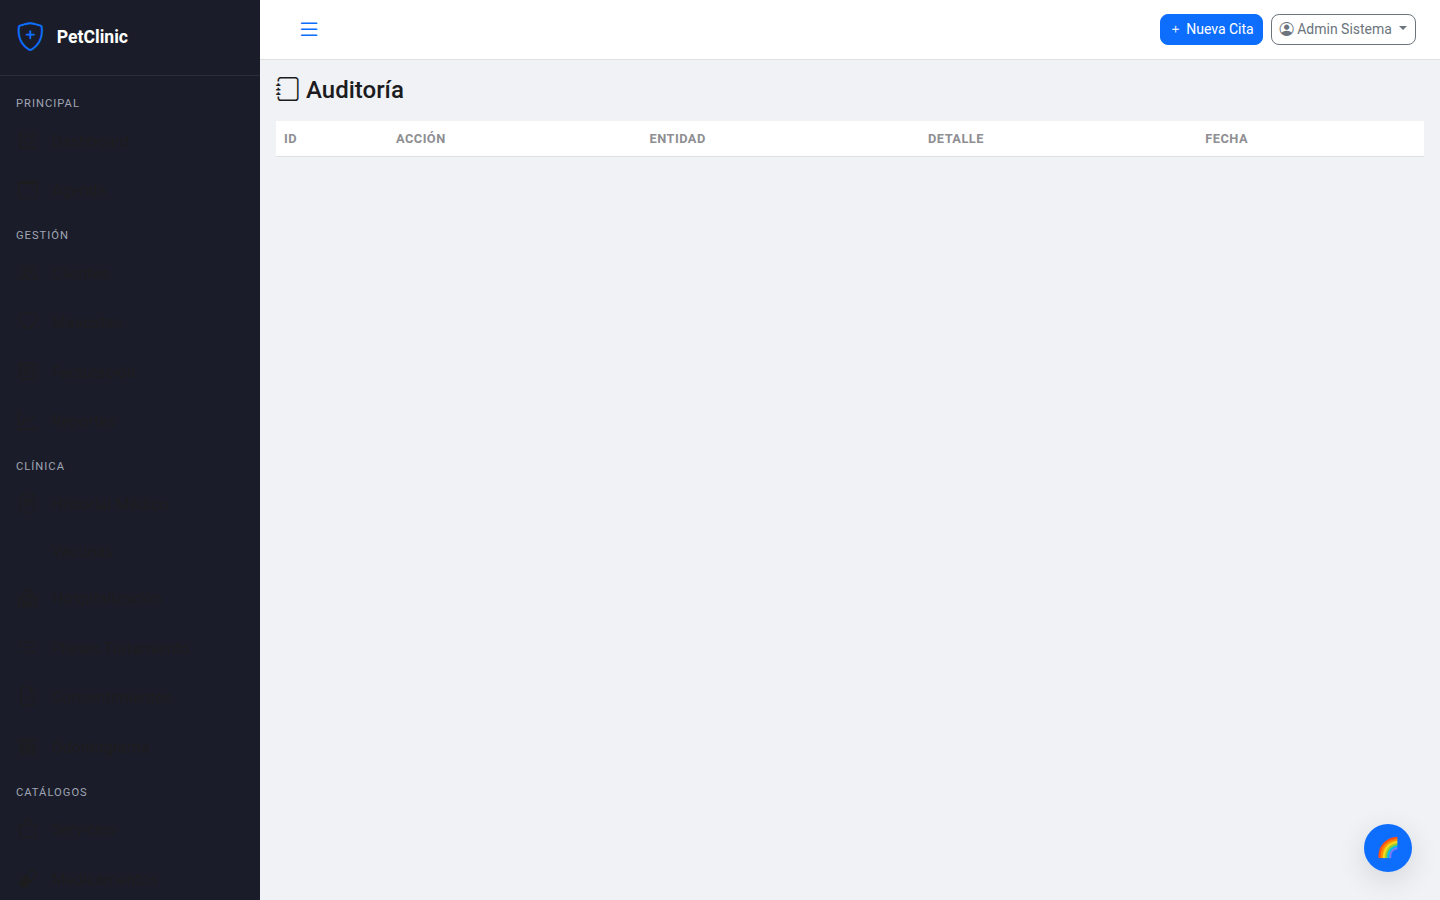
\includegraphics[width=0.9\textwidth]{images/17-auditoria}
    \caption{Registro de auditor\'ia con detalle de acciones por usuario}
    \label{fig:auditoria}
\end{figure}

\section{Protecci\'on de Contrase\~nas}

Todas las contrase\~nas se almacenan usando BCrypt mediante \texttt{BCryptPasswordEncoder} de Spring Security, con factor de costo 10 (10 rondas de hashing). El \texttt{PasswordEncoder} se define como un bean en \texttt{SecurityConfig}:

\begin{lstlisting}[language=Java]
@Bean
public PasswordEncoder passwordEncoder() {
    return new BCryptPasswordEncoder();
}
\end{lstlisting}

\section{CORS}

Configuraci\'on que permite peticiones desde cualquier origen para desarrollo, con soporte para credenciales:

\begin{lstlisting}[language=Java, caption=Configuraci\'on CORS]
@Bean
public WebMvcConfigurer corsConfigurer() {
    return new WebMvcConfigurer() {
        @Override
        public void addCorsMappings(CorsRegistry registry) {
            registry.addMapping("/api/**")
                .allowedOriginPatterns("*")
                .allowedMethods("GET", "POST", "PUT", "DELETE", "OPTIONS")
                .allowedHeaders("*")
                .allowCredentials(true);
        }
    };
}
\end{lstlisting}

\section{Protecci\'on CSRF}

CSRF est\'a deshabilitado porque la aplicaci\'on utiliza JWT stateless, lo que hace que los tokens CSRF sean innecesarios. La protecci\'on contra CSRF se logra mediante la validaci\'on del token JWT en cada petici\'on. En producci\'on, se recomienda agregar \texttt{HttpOnly} y \texttt{Secure} a las cookies si se usan, pero dado que el token se almacena en \texttt{localStorage} del navegador, la protecci\'on principal es contra XSS.
